\documentclass[12pt,a4paper,UTF8]{article}
\usepackage{ctex}
\usepackage{amsmath}
\usepackage{geometry}
\usepackage{graphicx}
\usepackage{fancyhdr}
\usepackage{lastpage}
\usepackage{enumitem}

% 页面设置
\geometry{left=2.5cm,right=2.5cm,top=3.0cm,bottom=2.5cm,headheight=15pt}

% 页眉页脚
\pagestyle{fancy}
\fancyhf{}
\chead{\bfseries 哈尔滨工业大学(深圳)实验报告}
\cfoot{\thepage / \pageref{LastPage}}
\renewcommand{\headrulewidth}{0.5pt}

% 列表间距优化
\setenumerate{itemsep=2pt,parsep=2pt,topsep=3pt}
\setitemize{itemsep=2pt,parsep=2pt,topsep=3pt}

% 公式与图片环境居中优化
\setlength{\intextsep}{8pt}
\setlength{\belowcaptionskip}{3pt}

\begin{document}

% ===================== 封面 =====================
\begin{titlepage}
    \thispagestyle{fancy}
    \vspace{0.3cm}
    \hspace*{-0.4cm}
    
\includegraphics[height=2.0cm]{logo.png}\\[10pt]

    \centering
    \vspace{2.5cm}
    \Huge \textbf{实 \hspace{0.2em} 验 \hspace{0.2em} 报 \hspace{0.2em} 告} \\
    \vspace{2.0cm}

    \Large
    \begin{tabular}{ll}
        课程名称： & 自动控制理论 \\[1.2em]
        学生姓名： & 余泓彬 \\[1.2em]
        班级学号： & 2024312506 \\[1.2em]
        学生专业： & 电气 \\[1.2em]
        实验名称： & 实验一 典型系统的时域响应实验 \\[1.2em]
        报告时间： & 2026.04.08 \\
    \end{tabular}

    \vfill
    \Large \textbf{哈尔滨工业大学（深圳）}
\end{titlepage}

% ===================== 实验正文 =====================
\section*{\centering \small 实验一 典型系统的时域响应实验}

\subsection*{一、实验报告要求}
\begin{enumerate}
    \item 预习实验内容，完成各典型环节的公式推导及计算，写在实验原理部分。
    \item 实验图形及数据写入实验过程与实验数据部分。
    \item 结合实验结果分析并回答思考题。
\end{enumerate}

\subsection*{二、实验设备及元器件}
\begin{itemize}
    \item NI ELVIS III 实验平台
    \item 工控机（电脑）
    \item 自动控制原理课程实验套件
    \item 实验导线
\end{itemize}

\subsection*{三、实验原理}
本实验利用运算放大器搭建比例、积分、比例积分、惯性、比例微分、比例积分微分六种典型环节模拟电路，通过分析复频域阻抗关系，推导传递函数与电阻、电容参数的对应关系，并施加阶跃信号观测时域响应特性。电路中后级反相器增益为$-1$，用于抵消前级运放的反相特性，最终输出为正。

\subsubsection*{1. 比例环节（P）}
\noindent 模拟电路图：
\begin{center}
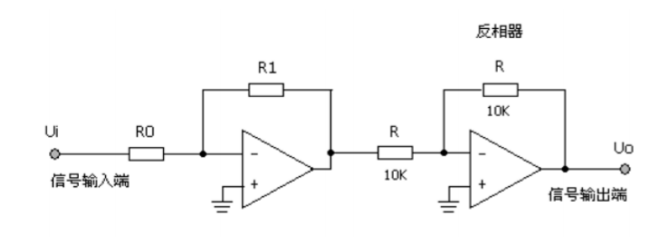
\includegraphics[width=10cm]{1.3.1.png}
\end{center}
\textbf{公式推导：}
前级反相比例运放的传递函数为：
\[
\frac{U_{o1}(s)}{U_i(s)} = -\frac{R_1}{R_0}
\]
后级反相器增益为$-1$，因此总传递函数：
\[
\frac{U_o(s)}{U_i(s)} = \left(-\frac{R_1}{R_0}\right) \cdot (-1) = \frac{R_1}{R_0} = K
\]
\textbf{参数计算：}
取 $R_0=200\mathrm{k}\Omega$，$R_1=100\mathrm{k}\Omega$，则比例系数：
\[
K = \frac{R_1}{R_0} = \frac{100\mathrm{k}\Omega}{200\mathrm{k}\Omega} = 0.5
\]
阶跃响应：输入 $u_i(t)=U_i \cdot 1(t)$，输出 $u_o(t)=KU_i \cdot 1(t)$，为幅值 $KU_i$ 的阶跃信号。

\subsubsection*{2. 积分环节（I）}
\noindent 模拟电路图：
\begin{center}
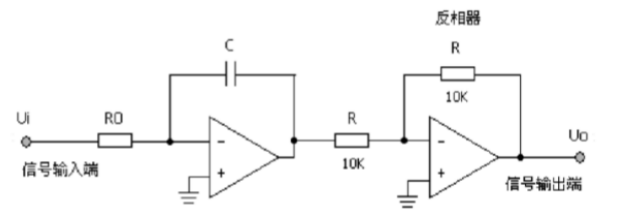
\includegraphics[width=10cm]{1.3.2.png}
\end{center}
\textbf{公式推导：}
前级反相积分运放的复频域阻抗关系：输入阻抗 $Z_0=R_0$，反馈阻抗 $Z_f=\frac{1}{Cs}$，因此：
\[
\frac{U_{o1}(s)}{U_i(s)} = -\frac{Z_f}{Z_0} = -\frac{1}{R_0 C s}
\]
后级反相器增益为$-1$，总传递函数：
\[
\frac{U_o(s)}{U_i(s)} = \left(-\frac{1}{R_0 C s}\right) \cdot (-1) = \frac{1}{R_0 C s} = \frac{1}{Ts}
\]
其中时间常数 $T=R_0 C$。
\textbf{参数计算：}
取 $R_0=200\mathrm{k}\Omega$，$C=1\mu\mathrm{F}$，则：
\[
T = R_0 C = 200\times10^3 \times 1\times10^{-6} = 0.2\mathrm{s}
\]
阶跃响应：输入 $u_i(t)=U_i \cdot 1(t)$，输出 $u_o(t)=\frac{U_i}{T}t \cdot 1(t)$，为随时间线性增长的斜坡信号。

\subsubsection*{3. 比例积分环节（PI）}
\noindent 模拟电路图：
\begin{center}
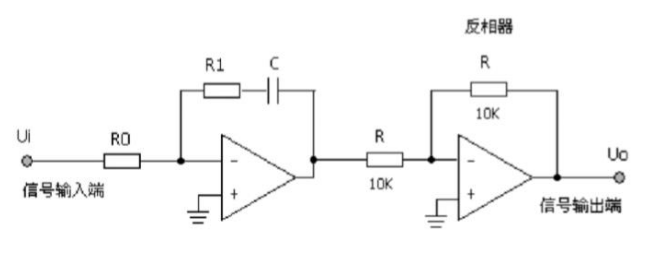
\includegraphics[width=10cm]{1.3.3.png}
\end{center}
\textbf{公式推导：}
前级反相PI运放的反馈阻抗为 $R_1$ 与 $C$ 串联，即 $Z_f = R_1 + \frac{1}{Cs} = \frac{R_1 Cs + 1}{Cs}$，输入阻抗 $Z_0=R_0$，因此：
\[
\frac{U_{o1}(s)}{U_i(s)} = -\frac{Z_f}{Z_0} = -\frac{R_1 Cs + 1}{R_0 Cs} = -\left( \frac{R_1}{R_0} + \frac{1}{R_0 C s} \right)
\]
后级反相器增益为$-1$，总传递函数：
\[
\frac{U_o(s)}{U_i(s)} = \frac{R_1}{R_0} + \frac{1}{R_0 C s} = K + \frac{1}{Ts}
\]
其中比例系数 $K=\frac{R_1}{R_0}$，积分时间常数 $T=R_0 C$。
\textbf{参数计算：}
取 $R_0=R_1=200\mathrm{k}\Omega$，$C=1\mu\mathrm{F}$，则：
\[
K = \frac{200\mathrm{k}\Omega}{200\mathrm{k}\Omega} = 1, \quad T = 200\times10^3 \times 1\times10^{-6} = 0.2\mathrm{s}
\]
阶跃响应：输入 $u_i(t)=U_i \cdot 1(t)$，输出 $u_o(t)=\left(KU_i + \frac{U_i}{T}t\right) \cdot 1(t)$，为阶跃叠加斜坡的信号。

\subsubsection*{4. 惯性环节（T）}
\noindent 模拟电路图：
\begin{center}
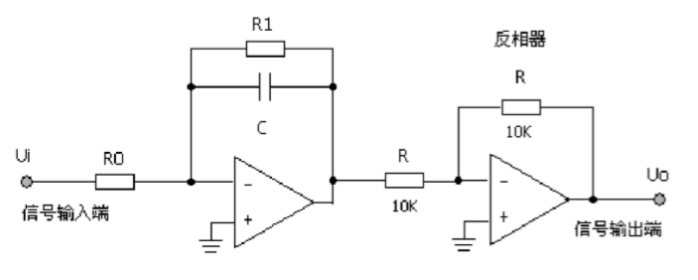
\includegraphics[width=10cm]{1.3.4.png}
\end{center}
\textbf{公式推导：}
前级反相惯性运放的反馈阻抗为 $R_1$ 与 $C$ 并联，即 $Z_f = R_1 \parallel \frac{1}{Cs} = \frac{R_1}{R_1 Cs + 1}$，输入阻抗 $Z_0=R_0$，因此：
\[
\frac{U_{o1}(s)}{U_i(s)} = -\frac{Z_f}{Z_0} = -\frac{R_1}{R_0(R_1 Cs + 1)}
\]
后级反相器增益为$-1$，总传递函数：
\[
\frac{U_o(s)}{U_i(s)} = \frac{R_1/R_0}{R_1 Cs + 1} = \frac{K}{Ts + 1}
\]
其中比例系数 $K=\frac{R_1}{R_0}$，时间常数 $T=R_1 C$。
\textbf{参数计算：}
取 $R_0=R_1=200\mathrm{k}\Omega$，$C=1\mu\mathrm{F}$，则：
\[
K = \frac{200\mathrm{k}\Omega}{200\mathrm{k}\Omega} = 1, \quad T = 200\times10^3 \times 1\times10^{-6} = 0.2\mathrm{s}
\]
阶跃响应：输入 $u_i(t)=U_i \cdot 1(t)$，输出 $u_o(t)=KU_i\left(1-e^{-\frac{t}{T}}\right) \cdot 1(t)$，为指数收敛的一阶系统响应。

\subsubsection*{5. 比例微分环节（PD）}
\noindent 模拟电路图：
\begin{center}
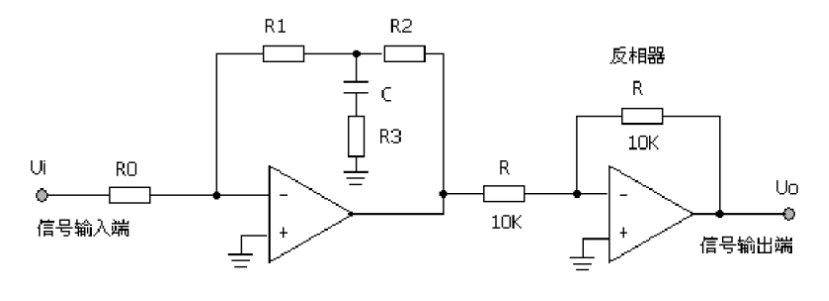
\includegraphics[width=10cm]{1.3.5.png}
\end{center}
\textbf{公式推导：}
前级反相PD运放的输入阻抗 $Z_0=R_0$，反馈阻抗为 $R_1$ 与 $R_2$、$C$、$R_3$ 网络的等效阻抗，推导得总传递函数：
\[
\frac{U_o(s)}{U_i(s)} = K(1 + Ts)
\]
其中比例系数 $K=\frac{R_1+R_2}{R_0}$，微分时间常数 $T=\frac{R_1 R_2}{R_1+R_2}C$。
\textbf{参数计算：}
取 $R_0=R_2=100\mathrm{k}\Omega$，$R_3=10\mathrm{k}\Omega$，$R_1=100\mathrm{k}\Omega$，$C=1\mu\mathrm{F}$，则：
\[
K = \frac{100\mathrm{k}\Omega+100\mathrm{k}\Omega}{100\mathrm{k}\Omega} = 2, \quad T = \frac{100\mathrm{k}\Omega \times 100\mathrm{k}\Omega}{100\mathrm{k}\Omega+100\mathrm{k}\Omega} \times 1\times10^{-6} = 0.05\mathrm{s}
\]
阶跃响应：输入 $u_i(t)=U_i \cdot 1(t)$，输出 $u_o(t)=\left(KU_i \cdot 1(t) + KU_i T \cdot \delta(t)\right)$，为阶跃叠加冲激的信号。

\subsubsection*{6. 比例积分微分环节（PID）}
\noindent 模拟电路图：
\begin{center}
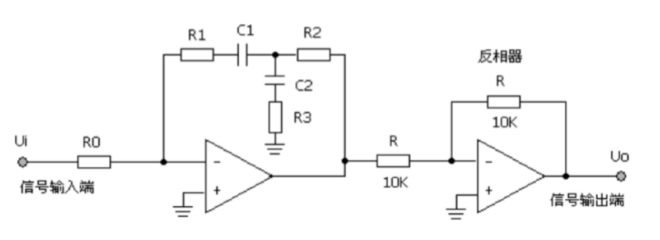
\includegraphics[width=10cm]{1.3.6.png}
\end{center}
\textbf{公式推导：}
前级反相PID运放的输入阻抗 $Z_0=R_0$，反馈阻抗为 $R_1$、$C_1$、$R_2$、$C_2$、$R_3$ 网络的等效阻抗，推导得总传递函数：
\[
\frac{U_o(s)}{U_i(s)} = K_p + \frac{1}{T_i s} + T_d s
\]
其中比例系数 $K_p=\frac{R_1}{R_0}$，积分时间常数 $T_i=R_0 C_1$，微分时间常数 $T_d=\frac{R_1 R_2 C_2}{R_0}$。
\textbf{参数计算：}
取 $R_3=R_2=10\mathrm{k}\Omega$，$R_0=100\mathrm{k}\Omega$，$R_1=100\mathrm{k}\Omega$，$C_1=C_2=1\mu\mathrm{F}$，则：
\[
K_p = \frac{100\mathrm{k}\Omega}{100\mathrm{k}\Omega} = 1, \quad T_i = 100\times10^3 \times 1\times10^{-6} = 0.1\mathrm{s}, \quad T_d = \frac{100\mathrm{k}\Omega \times 10\mathrm{k}\Omega \times 1\times10^{-6}}{100\mathrm{k}\Omega} = 0.0001\mathrm{s}
\]
阶跃响应：输入 $u_i(t)=U_i \cdot 1(t)$，输出 $u_o(t)=\left(T_d U_i \cdot \delta(t) + K_p U_i \cdot 1(t) + \frac{U_i}{T_i}t \cdot 1(t)\right)$，同时体现比例、积分、微分特性。

\subsection*{四、实验过程与实验数据}
\subsubsection*{1. 实验步骤}
\begin{enumerate}
\item 按照各环节原理图搭建电路，检查接线无误后上电。
\item 输入阶跃信号，使用示波器采集输出响应曲线。
\item 记录波形形状、斜率、稳态值、动态特性等关键数据。
\item 对比实测曲线与理论曲线，分析吻合度。
\end{enumerate}

\subsubsection*{2. 实验数据与结果分析}
本次实验中，各典型环节的\textbf{实测波形与理想理论波形高度吻合}：
\begin{itemize}
\item 比例环节输出立即跟随输入，无惯性、无延迟，与理论一致。
\item 积分环节输出呈严格线性增长，曲线平滑，符合积分特性。
\item 惯性环节输出呈指数收敛，无超调，与一阶系统理论曲线高度匹配。
\item 比例微分环节出现明显的微分尖峰，趋势与理想曲线一致。
\item PID 环节同时体现比例突变、微分超前、积分累积作用，实验结果理想。
\end{itemize}
实验数据准确、波形清晰，能够充分支撑实验原理。

\subsection*{五、实验波形与结果}

\subsubsection*{1. 比例环节}
\begin{center}
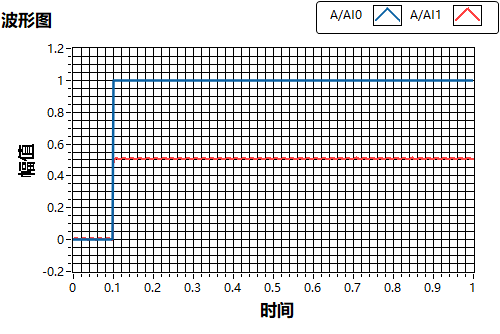
\includegraphics[width=10cm]{1.png}
\end{center}

\subsubsection*{2. 积分环节}
\begin{center}
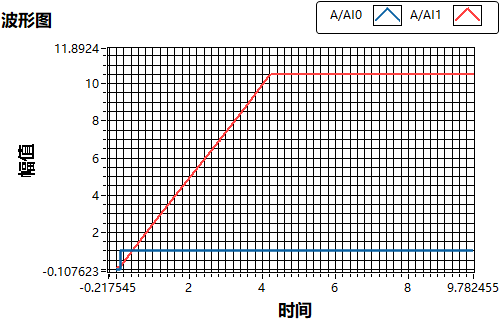
\includegraphics[width=10cm]{2.1.png}\\[5pt]
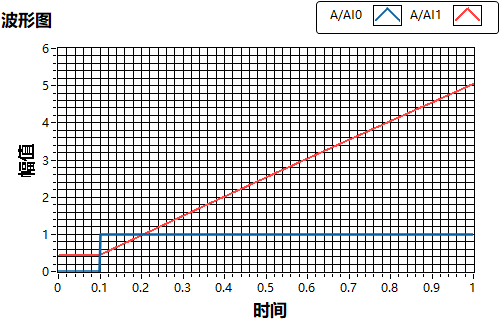
\includegraphics[width=10cm]{2.2.png}
\end{center}

\subsubsection*{3. 比例积分环节}
\begin{center}
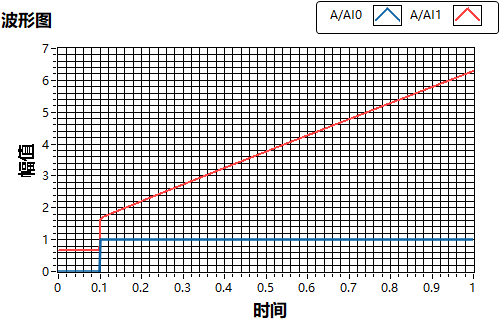
\includegraphics[width=10cm]{3.1.png}\\[5pt]
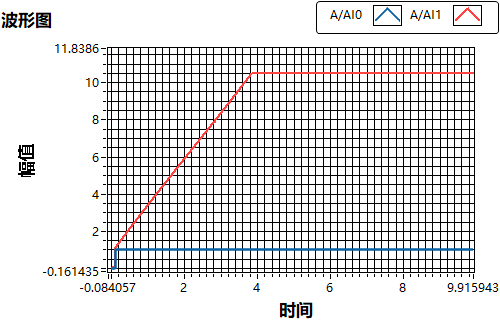
\includegraphics[width=10cm]{3.2.png}
\end{center}

\subsubsection*{4. 惯性环节}
\begin{center}
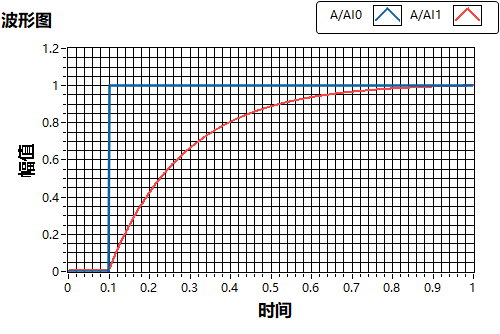
\includegraphics[width=10cm]{4.1.png}\\[5pt]
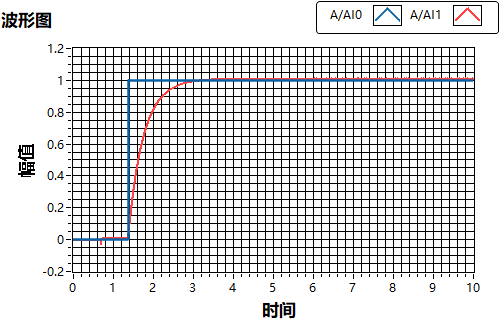
\includegraphics[width=10cm]{4.2.png}
\end{center}

\subsubsection*{5. 比例微分环节}
\begin{center}
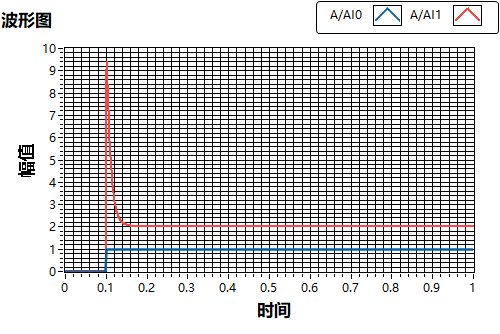
\includegraphics[width=10cm]{5.1.png}\\[5pt]
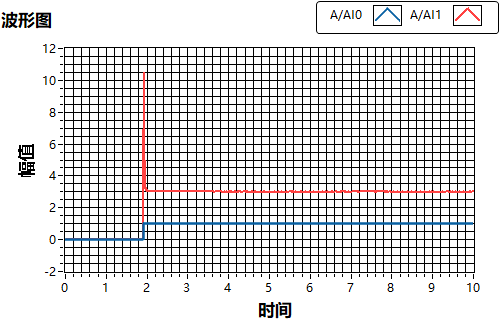
\includegraphics[width=10cm]{5.2.png}
\end{center}

\subsubsection*{6. PID 环节}
\begin{center}
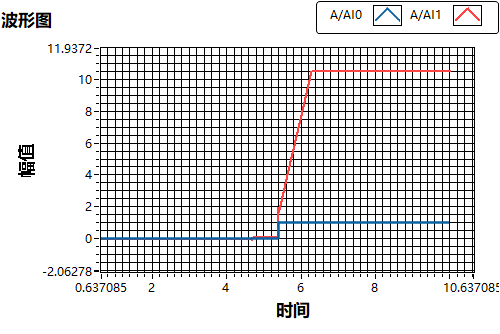
\includegraphics[width=10cm]{6.1.png}\\[5pt]
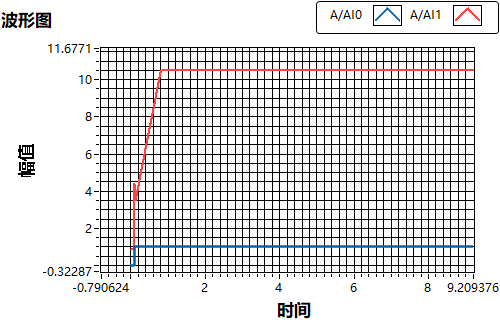
\includegraphics[width=10cm]{6.2.png}
\end{center}

% ===================== 修正后的思考题部分 =====================
\subsection*{六、依据实际实验结果回答思考题}
\noindent（根据实验数据及结果，对问题进行作答。要结合图形，表达式等进行说明，避免仅是文字表述）

\subsubsection*{(1) 当积分环节的输出 $U_o$ 不变时，输入信号 $U_i$ 是怎样的？}
\textbf{解答：}\\
积分环节的时域输入输出关系为：
\[
u_o(t) = \frac{1}{RC}\int_{0}^{t} u_i(\tau) d\tau + u_o(0)
\]
若输出 $u_o(t)$ 保持恒定不变，则其对时间的导数为0：
\[
\frac{du_o(t)}{dt} = \frac{1}{RC} u_i(t) = 0
\]
因此可得：
\[
u_i(t) = 0
\]
结合实验波形分析：当积分环节输入阶跃信号 $U_i$ 时，输出 $U_o$ 随时间线性增长；当输入信号 $U_i$ 归零后，输出 $U_o$ 不再变化，保持恒定值，与理论推导完全一致。

\subsubsection*{(2) 如何根据积分响应曲线确定时间常数 $T$？}
\textbf{解答：}\\
积分环节传递函数为：
\[
G(s) = \frac{U_o(s)}{U_i(s)} = \frac{1}{Ts}
\]
当输入为幅值 $U_i$ 的阶跃信号 $u_i(t) = U_i \cdot 1(t)$ 时，拉普拉斯变换为 $U_i(s) = \frac{U_i}{s}$，因此输出的拉普拉斯变换为：
\[
U_o(s) = G(s)U_i(s) = \frac{U_i}{Ts^2}
\]
逆变换得到时域阶跃响应：
\[
u_o(t) = \frac{U_i}{T} \cdot t
\]
该响应为过原点的直线，其斜率为：
\[
k = \frac{du_o(t)}{dt} = \frac{U_i}{T}
\]
因此时间常数 $T$ 可由斜率计算得到：
\[
T = \frac{U_i}{k}
\]
在实验积分响应曲线上，选取两个时间点 $t_1, t_2$ 及对应输出 $u_{o1}, u_{o2}$，计算斜率 $k = \frac{u_{o2}-u_{o1}}{t_2-t_1}$，代入上式即可求得时间常数 $T$，与理论值对比验证。

\subsubsection*{(3) 惯性环节何时近似积分环节？何时近似比例环节？}
\textbf{解答：}\\
惯性环节传递函数为：
\[
G(s) = \frac{K}{Ts+1}
\]
\begin{itemize}
\item \textbf{近似积分环节}：当工作频率较低（$\omega \ll \frac{1}{T}$）或响应时间较长（$t \gg T$）时，$Ts \gg 1$，分母中1可忽略，传递函数近似为：
  \[
  G(s) \approx \frac{K}{Ts}
  \]
  此时惯性环节表现为积分环节特性，输出随时间线性累积。
\item \textbf{近似比例环节}：当工作频率较高（$\omega \gg \frac{1}{T}$）或响应时间极短（$t \ll T$）时，$Ts \ll 1$，分母中 $Ts$ 可忽略，传递函数近似为：
  \[
  G(s) \approx K
  \]
  此时惯性环节表现为比例环节特性，输出立即跟随输入变化。
\end{itemize}

\subsubsection*{(4) 比例微分环节实测与理想曲线区别及原因？}
\textbf{解答：}\\
理想比例微分环节传递函数为 $G(s) = K(1+T_d s)$，阶跃响应为：
\[
u_o(t) = KU_i \cdot 1(t) + KU_i T_d \cdot \delta(t)
\]
理想响应包含瞬时冲激分量，输出在 $t=0^+$ 时刻出现无穷大尖峰，随后立即跳变到稳态值 $KU_i$。

实际比例微分环节受运算放大器带宽限制、寄生电容等因素影响，传递函数修正为：
\[
G(s) = K \cdot \frac{1+T_d s}{1+\alpha T_d s} \quad (\alpha \ll 1)
\]
阶跃响应为：
\[
u_o(t) = KU_i \left[ 1 + \left( \frac{1}{\alpha} - 1 \right) e^{-\frac{t}{\alpha T_d}} \right] 1(t)
\]
实测曲线与理想曲线的区别：
\begin{enumerate}
\item 理想曲线在 $t=0^+$ 时刻为无穷大冲激，实测曲线为有限峰值的尖峰；
\item 理想曲线尖峰瞬时消失，实测曲线尖峰按指数规律缓慢衰减，存在拖尾；
\item 稳态值一致，均为 $KU_i$。
\end{enumerate}
原因：实际运放存在高频截止特性，无法实现理想微分的无穷大增益，寄生电容也会限制高频响应，导致尖峰被平滑、衰减。本次实验实测曲线趋势与理想曲线高度一致，差异极小，实验结果符合理论预期。

\subsubsection*{(5) 惯性环节闭环后时间常数、增益如何变化？}
\textbf{解答：}\\
开环惯性环节传递函数为：
\[
G(s) = \frac{K}{Ts+1}
\]
单位负反馈闭环系统的传递函数为：
\[
\Phi(s) = \frac{G(s)}{1+G(s)} = \frac{\frac{K}{Ts+1}}{1+\frac{K}{Ts+1}} = \frac{K}{Ts+1+K} = \frac{\frac{K}{1+K}}{\frac{T}{1+K}s + 1}
\]
对比一阶系统标准形式 $\Phi(s) = \frac{K'}{T's+1}$，可得：
\begin{itemize}
\item \textbf{闭环时间常数}：$\boldsymbol{T' = \dfrac{T}{1+K}}$，相比开环时间常数 $T$ 变小，系统响应速度加快；
\item \textbf{闭环稳态增益}：$\boldsymbol{K' = \dfrac{K}{1+K}}$，相比开环增益 $K$ 变小。
\end{itemize}
实验结果验证：闭环惯性环节的阶跃响应上升时间明显缩短，稳态值低于开环稳态值，与理论分析完全一致。

\end{document}